\section{Zielsetzung}
Das Ziel dieses Versuches ist das Verhalten des RC-Kreises in Hinsicht auf
Auf- und Entladevorgänge, Frequenzabhängigkeit der Amplitude und der Phasenverschiebung
und die Integration der eingegebenen Spannung zu untersuchen.


\section{Theorie}
\subsection{Relaxationsgleichung für RC-Kreis}
Durch das Entfernen des RC-Kreises aus seinem Anfangszustand kehrt
dieser nach
\begin{equation}
  A(t) = A(\infty) + [A(0)- A(\infty)]\cdot \text{exp(ct)}
  \label{eqn:1}
\end{equation}
nicht-periodisch in diesen zurück. Dabei beschreibt $A(\infty)$ den Endzustand.
Wobei die Frequenz durch
\begin{equation}
  \omega = 2\pi f
  \label{eqn:frequenz}
\end{equation}
gegeben ist.

\begin{figure}[H]
  \centering
  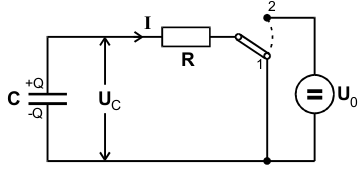
\includegraphics{content/images/pic1.png}
  \caption{Auf- und Entladung.}
  \label{pic:1}
\end{figure}


\subsubsection{Entladevorgang}
Der Kondersator besitzt die Ladungsmenge
\begin{equation}
  Q = U_\text{C}C
  \label{eqn:2}
\end{equation}
und eine Stromstärke von
\begin{equation}
  I = \frac{U_\text{C}}{R}.
  \label{eqn:3}
\end{equation}
Hierbei ist $U_\text{C}$ die Potentialdifferenz zwischen den
Kondensatorplatten.
Da die zeitliche Integration des Stroms die Ladungsmenge ist ergibt sich die Gleichung:
\begin{equation}
  \frac{\symup{d}\,Q}{\symup{d}\, t} = \frac{1}{RC}Q(t).
  \label{eqn:4}
\end{equation}
Unter der Bedingung, dass der Kondensator für $Q(\infty)$ komplett entladen ist
erhält man
\begin{equation}
 Q(t) =  Q(0) \text{exp}\left(\frac{-t}{RC}\right).
\label{eqn:5}
\end{equation}
Die verwendete Formel zur Bestimmung der Spannung ist :
\begin{equation}
  U(t)=U_0e^{-t/RC}.
  \label{eqn:entladen}
\end{equation}

\subsubsection{Aufladekurve}
Für die Aufladung sind die Randbedingungen $Q(0) = 0$ und $Q(\inf) = U_0 C$ wodurch
der Vorgang durch
\begin{equation}
  Q(t) = U_0C\, \left(1 - \text{exp}\left(\frac{-t}{RC}\right)\right)
  \label{eqn:6}
\end{equation}
beschrieben.
\begin{equation}
  \increment T = RC
  \label{eqn:7}
\end{equation}
gibt an wie schnell sich der Kondensator entlädt. Nach diesem Zeitraum
besitzt der Kondensator nach
\begin{equation}
\frac{Q(RC)}{Q(0)} = \frac{1}{e}
\label{eqn:8}
\end{equation}
noch die $\frac{1}{e}$-fache Ladungsmenge von $Q(0)$.
Die Aufladung wird nach
\begin{equation}
  U(t)=U_0\left(1-e^{-t/RC}\right)
  \label{eqn:aufladen}
\end{equation}
berechnet.

\subsection{Relaxation bei periodischer Auslenkung}
Der RC-Kreis zeigt für kleine Kreisfrequenzen $\omega<<\frac{1}{RC}$ keinerlei Phase
an, was bedeutet, dass $U$ dem $U_\text{C}$ entspricht.
Man beschreibt die Kondensatorspannung durch
\begin{equation}
  U_C(t)= A(\omega)\text{cos}(\omega t + \phi(\omega))
  \label{eqn:9}
\end{equation}
,mit dem zweiten Kirchhoff'schen Gesetz und Gl.\ref{eqn:3} und Gl.\ref{eqn:4}
ergibt sich
\begin{equation}
  U_0\text{cos(\omega t)} = -\text{A}\omega RC\sin{\omega t + \phi} + A(\omega)\text{cos}(\omega t + \phi).
\label{eqn:10}
\end{equation}
Da Gl.\ref{eqn:10} für alle t gelten muss, wodurch man $\omega t = \frac{\pi}{2}$
setzen kann. Daraus ergibt sich die Gleichung:
\begin{equation}
  \phi(\omega) = \text{arctan}(-\omega RC)
  \label{eqn:11}
\end{equation}
Aufgrunddessen ist die Phase für $\omega>>\frac{1}{RC}$ nahezu $\frac{\pi}{2}$, während
die Phase für $\omega=\frac{1}{RC}$ bei $\frac{\pi}{4}$ liegt.
Ebenso ergibt sich aus Gl.\ref{eqn:10} mit $\omega t + \phi$
\begin{equation}
  A(\omega)= -\frac{\text{sin}(\phi)}{\omega RC}U_0
  \label{eqn:12}
\end{equation}
,woraus abschließend eingesetzt folgende Gleichung für die
kreisfrequenzabhängige Amplitude gegeben ist:
\begin{equation}
  A(\omega) = \frac{U_0}{\sqrt{1 + w^2 R^2 C^2}}.
\label{eqn:13}
\end{equation}
Hieran ist zu erkennen, dass niedrigfrequente Spannungen
nahezu mit gleicher Amplitude durchkommen und hochfrequente Spannungen
mit sehr geringer Amplitude durchgelassen werden.
Die Phase wird durch
\begin{equation}
 \phi= \frac{a}{b}\cdot2\pi
 \end{equation}
bestimmt (siehe Abb.\ref{pic:4}) und es gilt
\begin{equation}
  \phi = \increment t \cdot\omega.
  \label{eqn:phasenberechnung}
\end{equation}
Somit wird die Amplitude nach
\begin{equation}
  A(\omega)=\frac{U_0}{\sqrt{1+\omega^2R^2C^2}}
  \label{eqn:amplitude}
\end{equation}
und die Phase durch
\begin{equation}
  \text{sin}(\phi)=\frac{\omega RC}{\sqrt{1+\omega^2R^2C^2}}
  \label{eqn:phase}
\end{equation}
berechnet.

\subsection{RC-Kreis als Integrator}

Unter der Bedingung, dass $\omega>>\frac{1}{RC}$ ist kann davon ausgegangen werden, dass
 die am Kondensator abfallende Spannung $U_\text{C}$ deutlich kleiner ist, als die Spannung
 die am Widerstand $U_\text{R}$ und die Gesamtspannung $U(t)$ abfällt. Dies ist die
 Bedingung die erfüllt sein muss
 um den RC-Kreis als Integrator verwenden zu können.
 Daraus ergibt sich die Näherung:
 \begin{equation}
   U(t) = R C \frac{\symup{d}\,U_\text{C}}{\symup{d}\,t}.
   \label{eqn:14}
\end{equation}
Diese lässt sich auch äquivalent zu
\begin{equation}
U_\text{C}(t)= \frac{1}{RC} \int_0^t U(\tau) \,\symup{d}\,\tau
\label{eqn:integral}
\end{equation}
umschreiben.

\subsection{Fehlerrechnung}
Verwendete Fehlerformel ist
\begin{equation}
  \text{Abweichung} = \left|\frac{x_\text{theoretisch}-x_\text{praktisch}}{x_\text{theoretisch}}\right|
  \label{eqn:abweichung}
\end{equation}
zur Berechnung der prozentualen Abweichung.
